\chapter{Synthetic Experiments}
\label{sec:synthetic}

This chapter describes experiments done on synthetic data to explore the learning performance of the methods described in the background section.

\section{Learning Setup}

This section describes implementation details of NCE and SGD, these are applicable for both the experiments in this chapter as well as those performed on real data, which will presented in subsequent chapters.

\subsection{Noise Distribution}

As mentioned in section \ref{sec:nce-practical}, there are several considerations when choosing the noise distribution. A log-modular distribution is a natural choice for the noise when learning the FLID model \citep{tschiatschek16learning}, and this distribution will also be used for the noise with FLDC and FFLDC models.

The parameters of a log-modular distribution can be estimated efficiently from data through MLE, as given by Equation \eqref{eq:modular-mle}. Also the partition function can be computed in closed form, as shown in Equation \eqref{eq:modular-z}. This makes the distribution a good candidate because it can be used efficiently for sampling as well as for computing the normalized probability of sets, i.e. $P_{n}(S)$ during the learning procedure.

\subsection{Initialization}

The log-modular model also provides a sensible initialization for vector $\mathbf{u}$ in the FLID and FLDC models. For FFLDC, the initialization for $\mathbf{a}$ is done by solving the linear system derived from the factorization in Equation \eqref{eq:ffldc-factorization-1}, this linear system is given by:

\begin{equation}
  \mathbf{a} = \mathbf{X}^{-1}\mathbf{u}
\end{equation}

Unfortunately, this system can be under/over-determined in many cases so an approximated solution must be used. The chosen method for finding this solution is Ridge regression which minimizes the squared error $\sum_{i \in S}(u_{i} - (\mathbf{X}\mathbf{a})_{i})^{2}$ with a regularization term on the $l_{2}$ norm of $\mathbf{a}$.

The weight matrices, e.g. $\mathbf{W}^{e}, \mathbf{B}$, are initialized with random values drawn from a uniform distribution $\mathcal{U} \sim [0, 0.001]$. These is the same initialization setting proposed by \citet{tschiatschek16learning}.

In the cases where AdaGrad is used, the accumulated gradient $\mathbf{G}$ is initialized with a constant value for each parameter $\gamma$, namely $G^{0}_{\gamma} = 0.01$.

\subsection{Learning rate}

When not using AdaGrad, the learning rate used in the experiments follows the power law mentioned in section \ref{sec:adagrad}, i.e.

\begin{equation}
  \eta(t) = \frac{\eta_{0}}{t^{p}}
\end{equation}

\subsection{Projection in SGD}

The weight matrices, e.g. $\mathbf{W}^{e}, \mathbf{B}$, are defined only for positive values. Therefore, they must be projected in each gradient step to ensure that the solution stays in the feasible space. This is done following the procedure proposed by \citet{tschiatschek16learning} which produces better results than simply clipping the values to 0. Let $\theta_{h}$ be an element of these matrices, e.g. $\theta_{h} = w^{e}_{i,d}$, then the projection is defined as:

\begin{equation}
  \theta_{h} = \begin{cases}
    \theta'_{h} & \text{if}\ \theta'_{h} \geq 0 \\
    \mathcal{U} \sim [0, 0.001] & \text{otherwise}
  \end{cases}
\end{equation}

Where $\theta'_{h}$ is the unnormalized parameter after the gradient update and $\mathcal{U} \sim [0, 0.001]$ means that the value is drawn from an uniform distribution between $[0, 0.001]$ as in the initialization.

\subsection{Termination Criteria}

The termination criteria for learning was the number of epochs, i.e. full passes over the data and noise samples.

\section{Example Datasets}

This section presents the results obtained after learning the datasets from the examples given for each model. For these experiments, the settings were:

\begin{itemize}
  \item 1000 samples of data drawn from the corresponding distribution, i.e. $|\mathcal{D}| = 1000$.
  \item 2000 noise samples, i.e. $\nu = 2$.
  \item 100 epochs.
  \item $\eta_{0}$ is 0.005 and $p = 0.1$ for the learning rate, without AdaGrad.
\end{itemize}

It is worth noting that the presented results for these experiments correspond to the best of multiple runs. It was observed that the learning algorithm does not always arrive to a good solution. This is because $g(\boldsymbol{\theta})$ is not a concave function and some initializations may lead to local maxima.

\subsection{FLID: Two Landmarks}

Recall the following characteristics about the dataset in Example \ref{sec:flid-toy}:

\begin{itemize}
  \item There are 3 elements, $h$, $s$, $f$.
  \item There are only 2 possible sets, $\{h,s\}$ and $\{h,f\}$. Both equally likely, i.e. $P(S) = 0.5$.
  \item A model can be constructed with a single diversity dimension, i.e. $L=1$.
\end{itemize}

After estimating the parameters from this data, the resulting utility vector and weight matrix are:

\begin{align*}
  \mathbf{u} = \left(5.42,2.82,2.79\right)^{\intercal} \\
  \mathbf{W}^{b} = \left(0.02, 6.10, 6.10\right)^{\intercal}
\end{align*}

This is a slightly different model from the one suggested in section \ref{sec:flid-toy}, however the normalized probability distribution for this model presented in Table \ref{tab:flid-toy-learned-probs} shows that it closely approximates the distribution.

\begin{table}
  \centering
  \caption{Learned distribution for Example \ref{sec:ffldc-toy}}
  \begin{tabular}{@{}ll@{}}
    \toprule
    $S$ & $P(S)$\\
    \midrule
    $\{h,s\}$ & $0.48$ \\
    $\{h,f\}$ & $0.47$ \\
    $\{h\}$ & $0.03$ \\
    $\{h,s,f\}$ & $0.02$ \\
    \bottomrule
  \end{tabular}
  \label{tab:flid-toy-learned-probs}
\end{table}

\subsection{FLDC: Two Non-overlapping Clusters}

Recall the following characteristics about the dataset in Example \ref{sec:fldc-toy}:

\begin{itemize}
  \item There are 4 items, i.e. $V = \{1,2,3,4\}$.
  \item There are only 2 possible sets, $\{1,2\}$ and $\{3,4\}$. Both equally likely, i.e. $P(S) = 0.5$.
  \item A model can be constructed with two diversity and two coherence dimensions, i.e. $L=2,K=2$.
\end{itemize}

Figure \ref{fig:fldc-toy-learned-weights} shows the resulting utility vector $\mathbf{u}$ and weight matrices $\mathbf{W}^{b}, \mathbf{W}^{e}$ after the learning procedure.

\begin{figure}
  \centering
  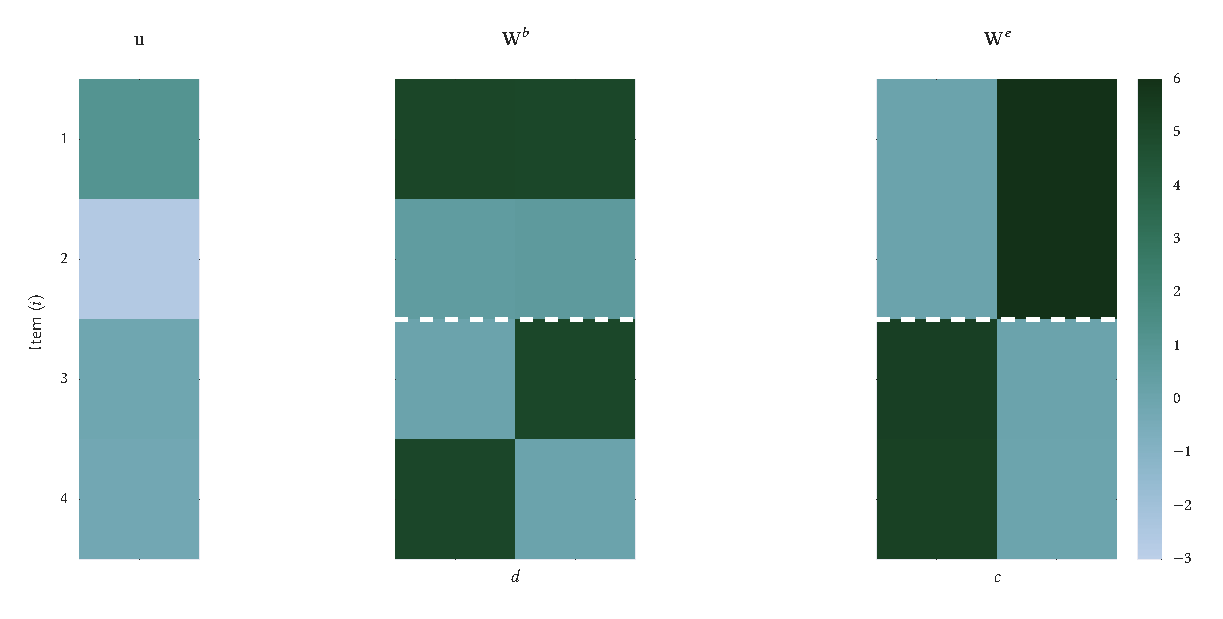
\includegraphics[width=\textwidth]{fldc_toy_example_learned_weights}
  \caption{Learned model for example \ref{sec:fldc-toy}. The white line divides the clusters described in the example.}
  \label{fig:fldc-toy-learned-weights}
\end{figure}

The model shown in the figure displays the desired properties of diversity between the clusters while having coherence between the items in each one. Despite being different from the proposed model in section \ref{sec:fldc-toy} it also approximately realizes the desired distribution.

\subsubsection{FFLDC: Rated Locations}

Recall the following characteristics about the dataset in Example \ref{sec:ffldc-toy}:

\begin{itemize}
  \item There are 6 items, i.e. $V = \{1,2,3,4,5,6\}$.
  \item The full distribution is related to the features and is given in Table \ref{tab:ffldc-toy-probs}.
  \item The proposed model has 2 diversity dimensions and one coherence dimension.
\end{itemize}

\begin{figure}
  \centering
  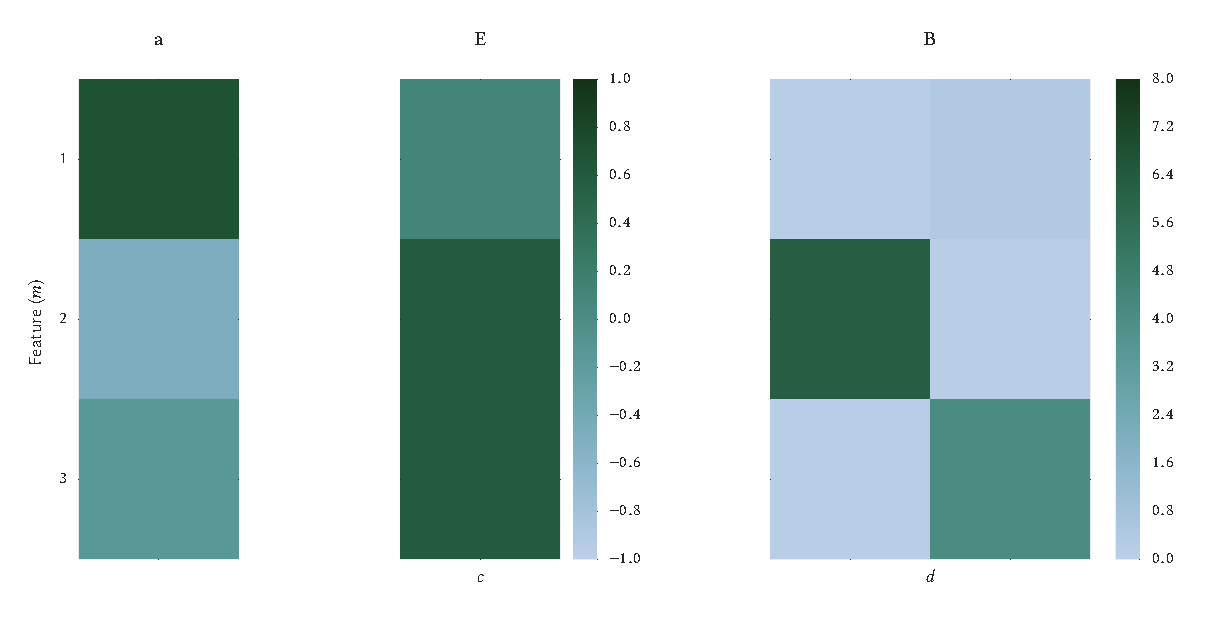
\includegraphics[width=\textwidth]{ffldc_toy_example_learned_weights}
  \caption{Learned model for example \ref{sec:ffldc-toy}}
  \label{fig:ffldc-toy-learned-weights}
\end{figure}

Figure \ref{fig:ffldc-toy-learned-weights} shows the resulting model after learning. Unfortunately, this model can be not as easily interpreted as the one proposed in figure \ref{fig:ffldc-toy-all-weights}, nevertheless it accurately models the distribution from the example thus showing the learning algorithm's ability to estimate a distribution using features.

\section{Learning rate sensitivity}

This section explores the learning rate's effect on the learning performance for the synthetic dataset from Example \ref{sec:ffldc-toy}.

The first experiment considers the stability of the optimization without AdaGrad as the learning rate increases. The settings are the same as for the previous experiments with the following additions:

\begin{itemize}
  \item $\eta_{0}$ is increased between $0.0005$ and $0.02$
  \item The learning is performed independently 8 times to obtain statistics on the results.
\end{itemize}

Figure \ref{fig:effects_eta_0} shows $g(\boldsymbol{\theta})$ during the optimization, each point corresponds to the mean value calculated after a given number of epochs and the error bars show the corresponding 95\% confidence interval for the mean.

\begin{figure}
  \centering
  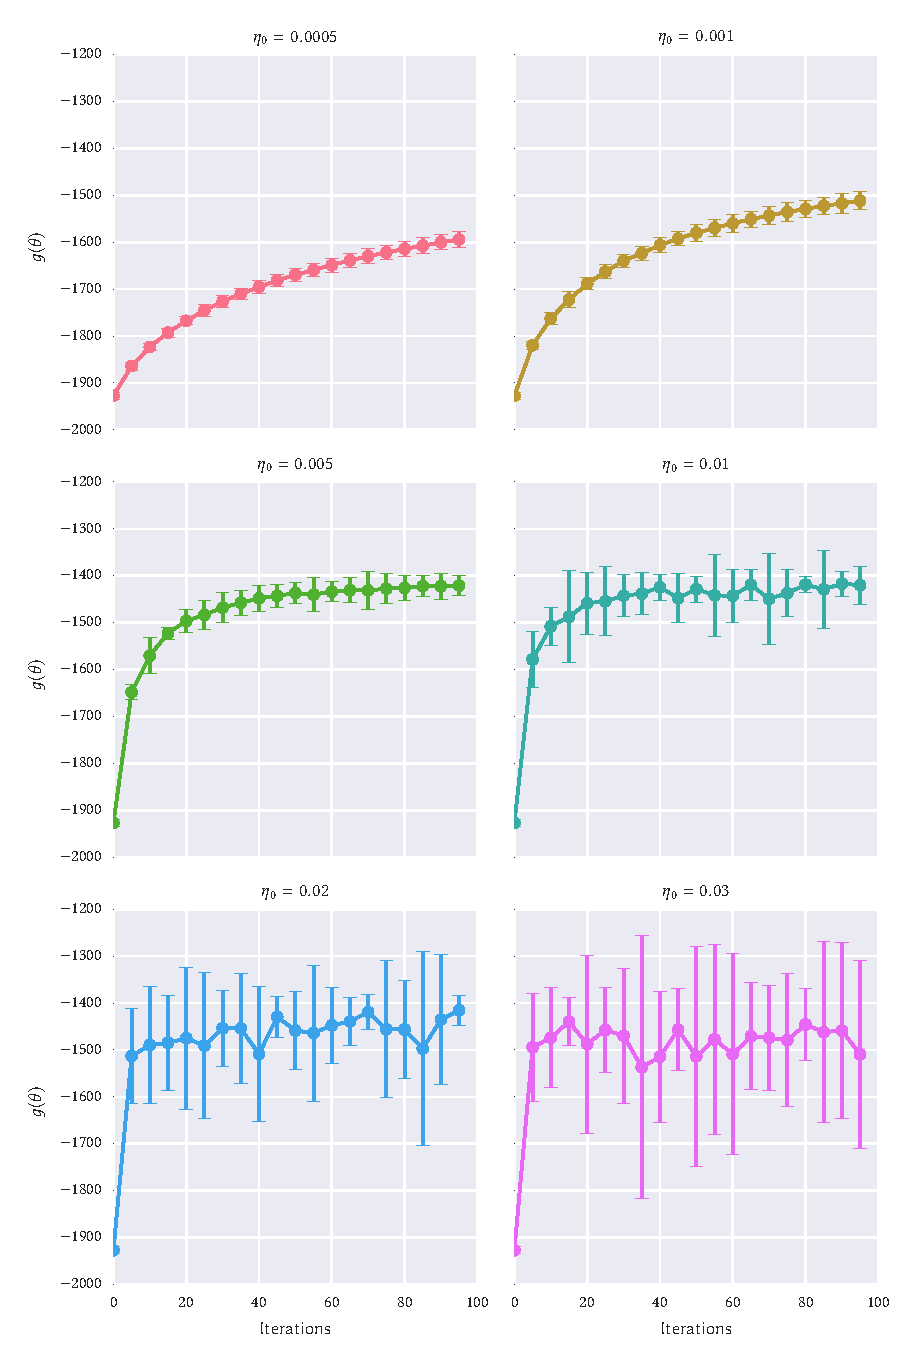
\includegraphics[width=\textwidth]{effects_eta_0_ffldc}
  \caption{Objective function for various values of $\eta_0$ without using AdaGrad.}
  \label{fig:effects_eta_0}
\end{figure}

The results in figure \ref{fig:effects_eta_0} show that for small values of $\eta_0$ the learning can be significantly slow and that large values of $\eta_0$ may lead to instability, as discussed in section \ref{sec:adagrad}. Concretely, for $\eta_{0} \leq 0.01$ the learning is slow but stable, while for $\eta_{0} \geq 0.01$ the objective value converges quickly but oscillates significantly. Fortunately, in the particular case of this synthetic dataset there exists a learning rate for which the objective function converges and is stable, i.e. $\eta_{0} = 0.005$ however this is not always the case for real data.

By contrast, figure \ref{fig:effects_adagrad} shows the objective function for $\eta_{0}$ between $0.005$ and $0.05$ after incorporating AdaGrad to the implementation. These results show that training with AdaGrad is stable for a larger range of $eta_0$.

\begin{figure}
  \centering
  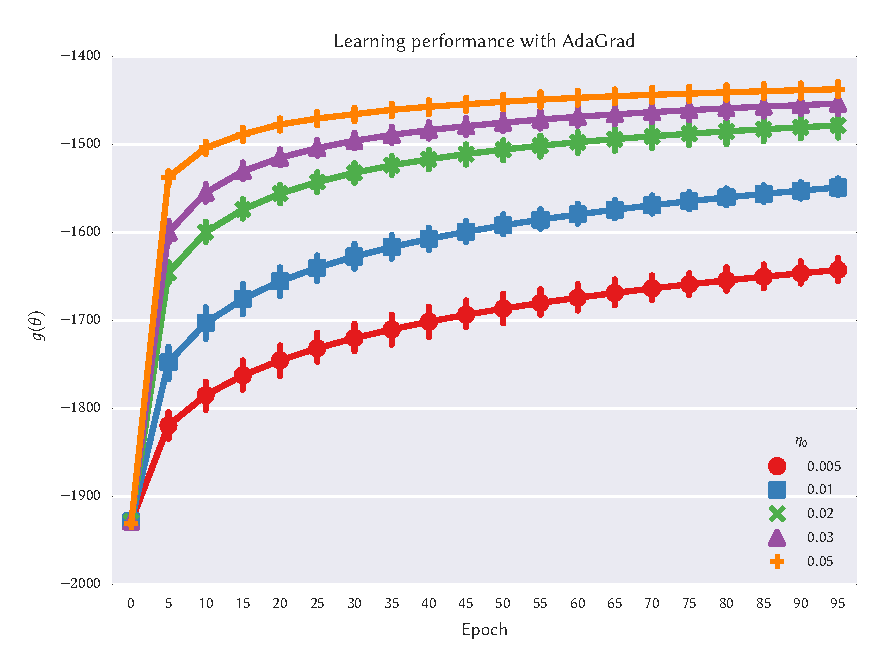
\includegraphics[width=\textwidth]{effects_eta_0_ffldc_adagrad}
  \caption{Objective function during learning for various values of $\eta_0$ with AdaGrad.}
  \label{fig:effects_adagrad}
\end{figure}

Finally, figure \ref{fig:comparison_adagrad_ffldc_toy} shows a direct comparison between training with and without AdaGrad using the best values of $\eta_0$ for each configuration. In this figure both algorithms converge to an optimal value, however it also shows that training with AdaGrad converges significantly faster while mantaining a stable mean. These combined results indicate that using AdaGrad is the best strategy for learning the FFLDC model.

\begin{figure}
  \centering
  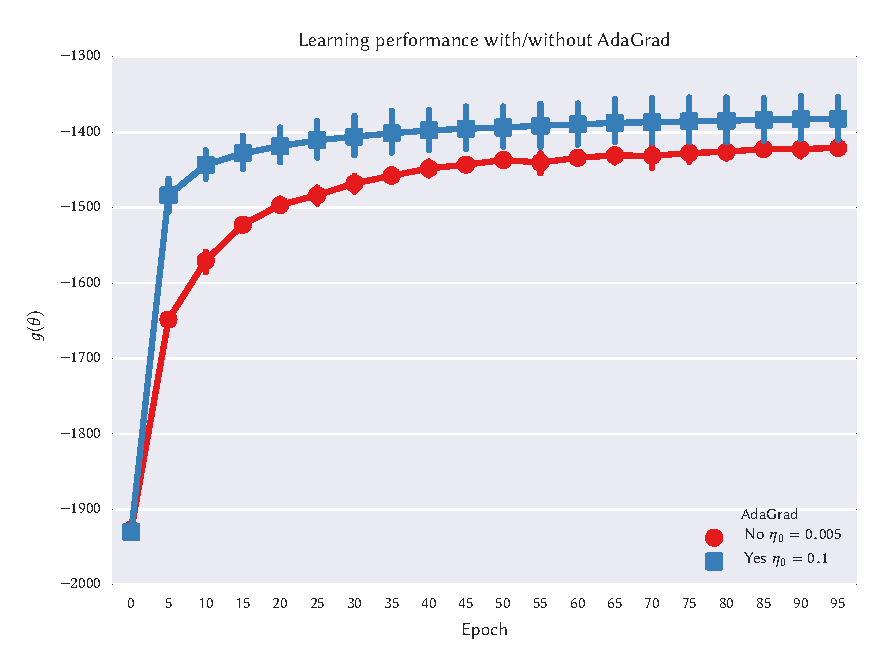
\includegraphics[width=\textwidth]{ffldc_adagrad_comparison}
  \caption{Comparison of learning performance with and without AdaGrad.}
  \label{fig:comparison_adagrad_ffldc_toy}
\end{figure}
